\section{Introduccion al proyecto Beerbot}
\label{introduccion_desarrollo}

En esta sección se presenta la parte central del trabajo, el proyecto Beerbot, acrónimo de Beer Extracting Environment Robot. Se trata de un sistema formado por un robot móvil con una pinza y una cámara situada sobre el escenario. La cámara se conectará con un ordenador, que será el encargado de ejecutar el algoritmo desarrollado, desde el procesamiento de la imagen a la planificación de la trayectoria y el control de alto nivel del robot. Este ordenador se comunicará con el microcontrolador del robot a través de un módulo bluetooth, enviándole la velocidad de giro de cada rueda.\\

\begin{figure}[H]
        \centering
        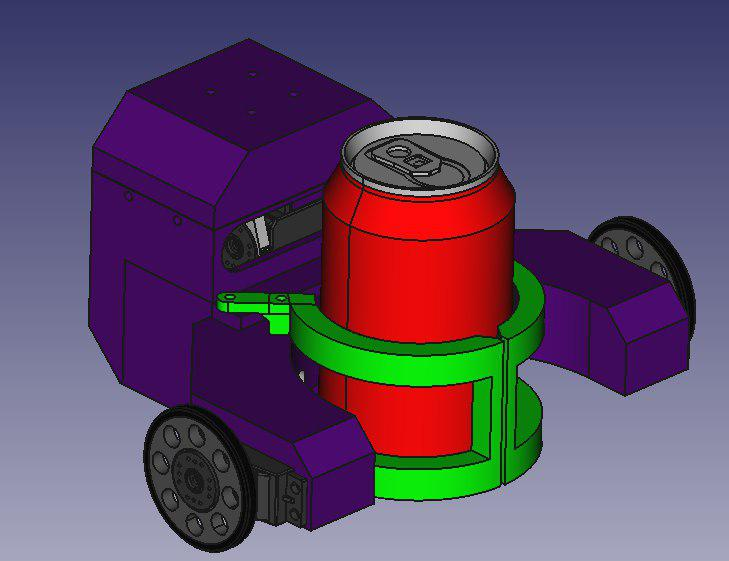
\includegraphics[width=0.4\textwidth]{images/robot.jpg}
        \caption{Modelo 3D del robot}
        \label{fig:robot}
\end{figure} 

\subsection{Objetivos}

El objetivo principal de este proyecto es desarrollar un robot que sea capaz de navegar por un entorno con obstáculos estáticos para localizar una lata, recogerla con la pinza y llevarla al punto inicial. Para ello se trabajará con algoritmos de procesamiento de imágenes, algoritmos de planificación de trayectorias, e impresión 3D, para la fabricación del robot.\\

Además de este objetivo, con este trabajo también se pretende diseñar una aplicación real y física que permita poner en práctica los conceptos adquiridos no solo en la asignatura en sí, si no a lo largo del máster. Se han llevado a cabo otros proyectos acerca de planificación, pero en entornos simulados, por lo que la fabricación del robot y el uso de un entorno real son la parte clave, ya que con esto se podrá estudiar como las características del entorno afecta a los resultados obtenidos.\\
 
Respecto a la parte de procesamiento de imágenes, el hecho de tener un escenario con iluminación no controlada obligará a tener que explorar diferentes alternativas para combatir los cambios de iluminación y poder conseguir los resultados esperados, especialmente en la etapa de segmentación de la imagen. Por otra parte, a diferencia de las simulaciones, el robot presentará errores de posición que será necesario corregir añadiendo un mecanismo de seguimiento de la trayectoria, para asegurarse que se llegue al punto al que realmente se está tratando de llegar.\\
 
\subsection{Funcionamiento del sistema}

El sistema funciona de la siguiente manera. El robot se sitúa en el escenario elegido, en un punto cualquiera. La cámara aérea captura una imagen del escenario, que se procesa para extraer de ella los obstáculos presentes en el entorno, la posición y orientación del robot y la posición del objetivo, es decir, la lata. Todos estos datos se envían al algoritmo de planificación, que muestrea el espacio libre por el que puede pasar el robot y calcula la ruta óptima por la que se pueda alcanzar el objetivo sin colisionar con los obstáculos. Conociendo los puntos por los que pasa la trayectoria, se va controlando la posición del robot en cada instante y se convierte la diferencia entre dicha posición y el siguiente punto del camino a comandos que le indiquen al robot la velocidad que debe llevar cada rueda. Una vez se alcanza una posición cercana a la lata, se abre la pinza, se coge la lata y el robot hace el mismo camino en la otra dirección (se supone que al ser un entorno estático, la trayectoria óptima debería seguir siendo la misma, además de simplificar el proceso, al ahorrarse un ciclo de planificación) hasta llegar al punto del que había partido, donde dejará la lata. En la siguiente sección de la memoria se comentarán más en detalle las diferentes partes del sistema.\\

\subsection{Escenario a utilizar}

Se va a trabajar sobre una pista cuadrada desarrollada para el concurso de robótica humanoide CEABOT. Tiene unas medidas de  y un suelo de color verde, que facilita las tareas de segmentación. Para los obstáculos, se han utilizado objetos diversos que se han encontrado en la zona de trabajo, ya que era lo que se tenía a mano. Además con esto se consigue otra cosa: mostrar que no es necesario que los obstáculos tengan un color, tamaño o forma determinada, ya que se pueden detectar como tal sin problema. En cuanto a la lata, tendrá un tamaño estándar, pero no es necesario que tenga un color determinado, lo que permite que el sistema no esté limitado a un único tipo de objetivo. En cuanto a la cámara, se han utilizado dos listones rígidos unidos por un cable como estructura para soportarla. En la figura \ref{fig:escenario} se puede observar el escenario durante la etapa de montaje de la estructura que soporta la cámara.\\

\begin{figure}[H]
        \centering
        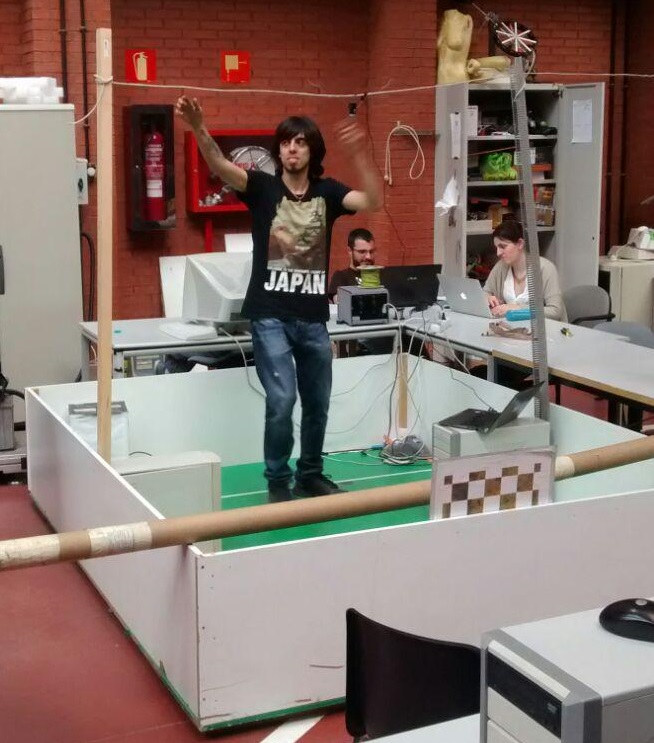
\includegraphics[width=0.4\textwidth]{images/escenario.jpg}
        \caption{Escenario empleado}
        \label{fig:escenario}
\end{figure} 

Esta solución presenta varios problemas, siendo uno bastante importante las vibraciones que se generan al temblar el cable. Esto se podría solucionar fabricando una estructura rígida que soporte mejor la cámara. Otro problema por utilizar este escenario, quizás el más grave de todos, es que está situado en una zona muy amplia que, a pesar de ser interior, recibe una gran cantidad de luz natural proveniente de grandes ventanas situadas en el techo, que unido a la luz artificial presente, provoca que no se consiga una iluminación constante a lo largo del día, generándose gran cantidad de sombras en algunas zonas, o brillos en otras (esto también se debe al tipo de suelo que presenta el entorno), lo que dificulta en gran medida el correcto procesamiento de la imagen.\\  